
\begin{figure}
    \centering
    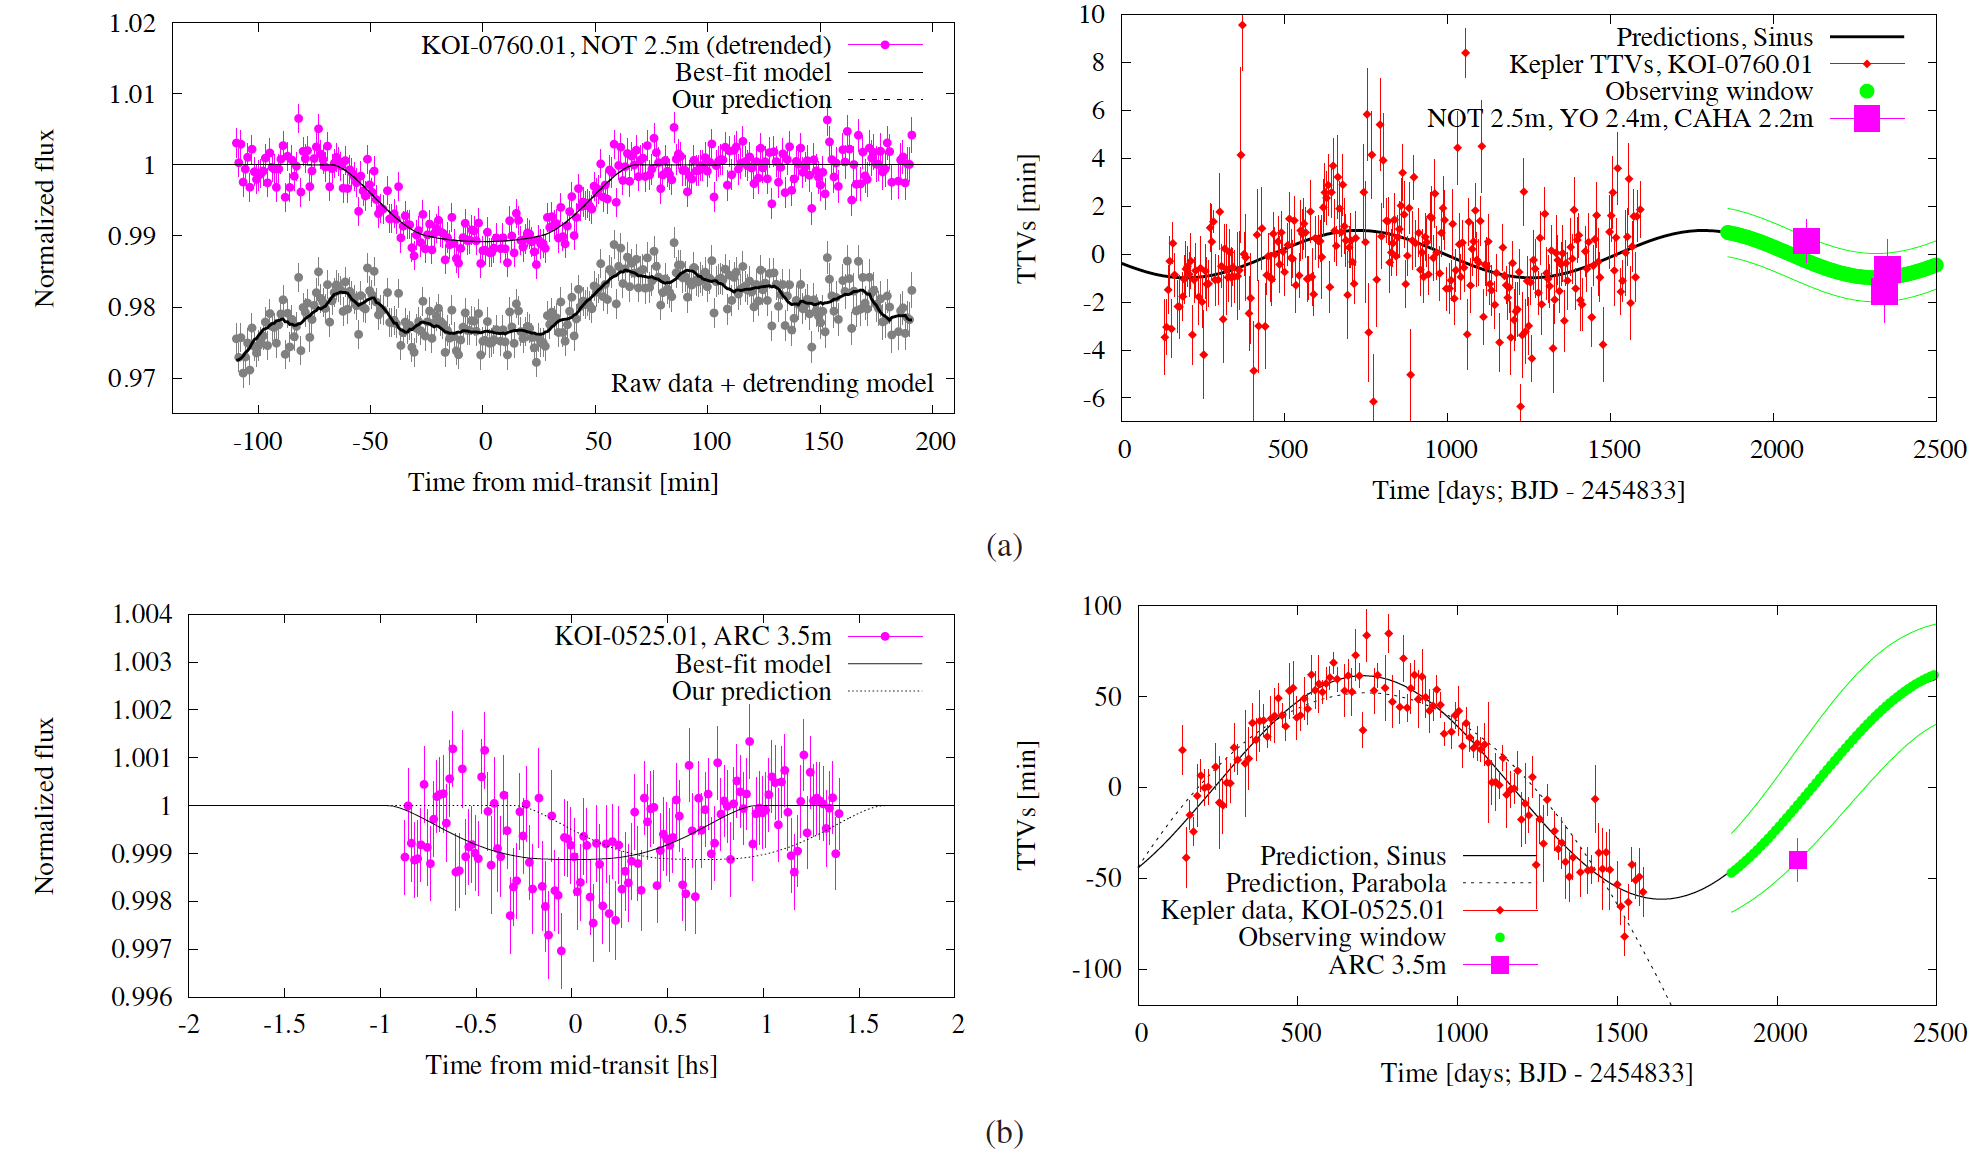
\includegraphics[scale=0.23]{koinet/caro1.png}
    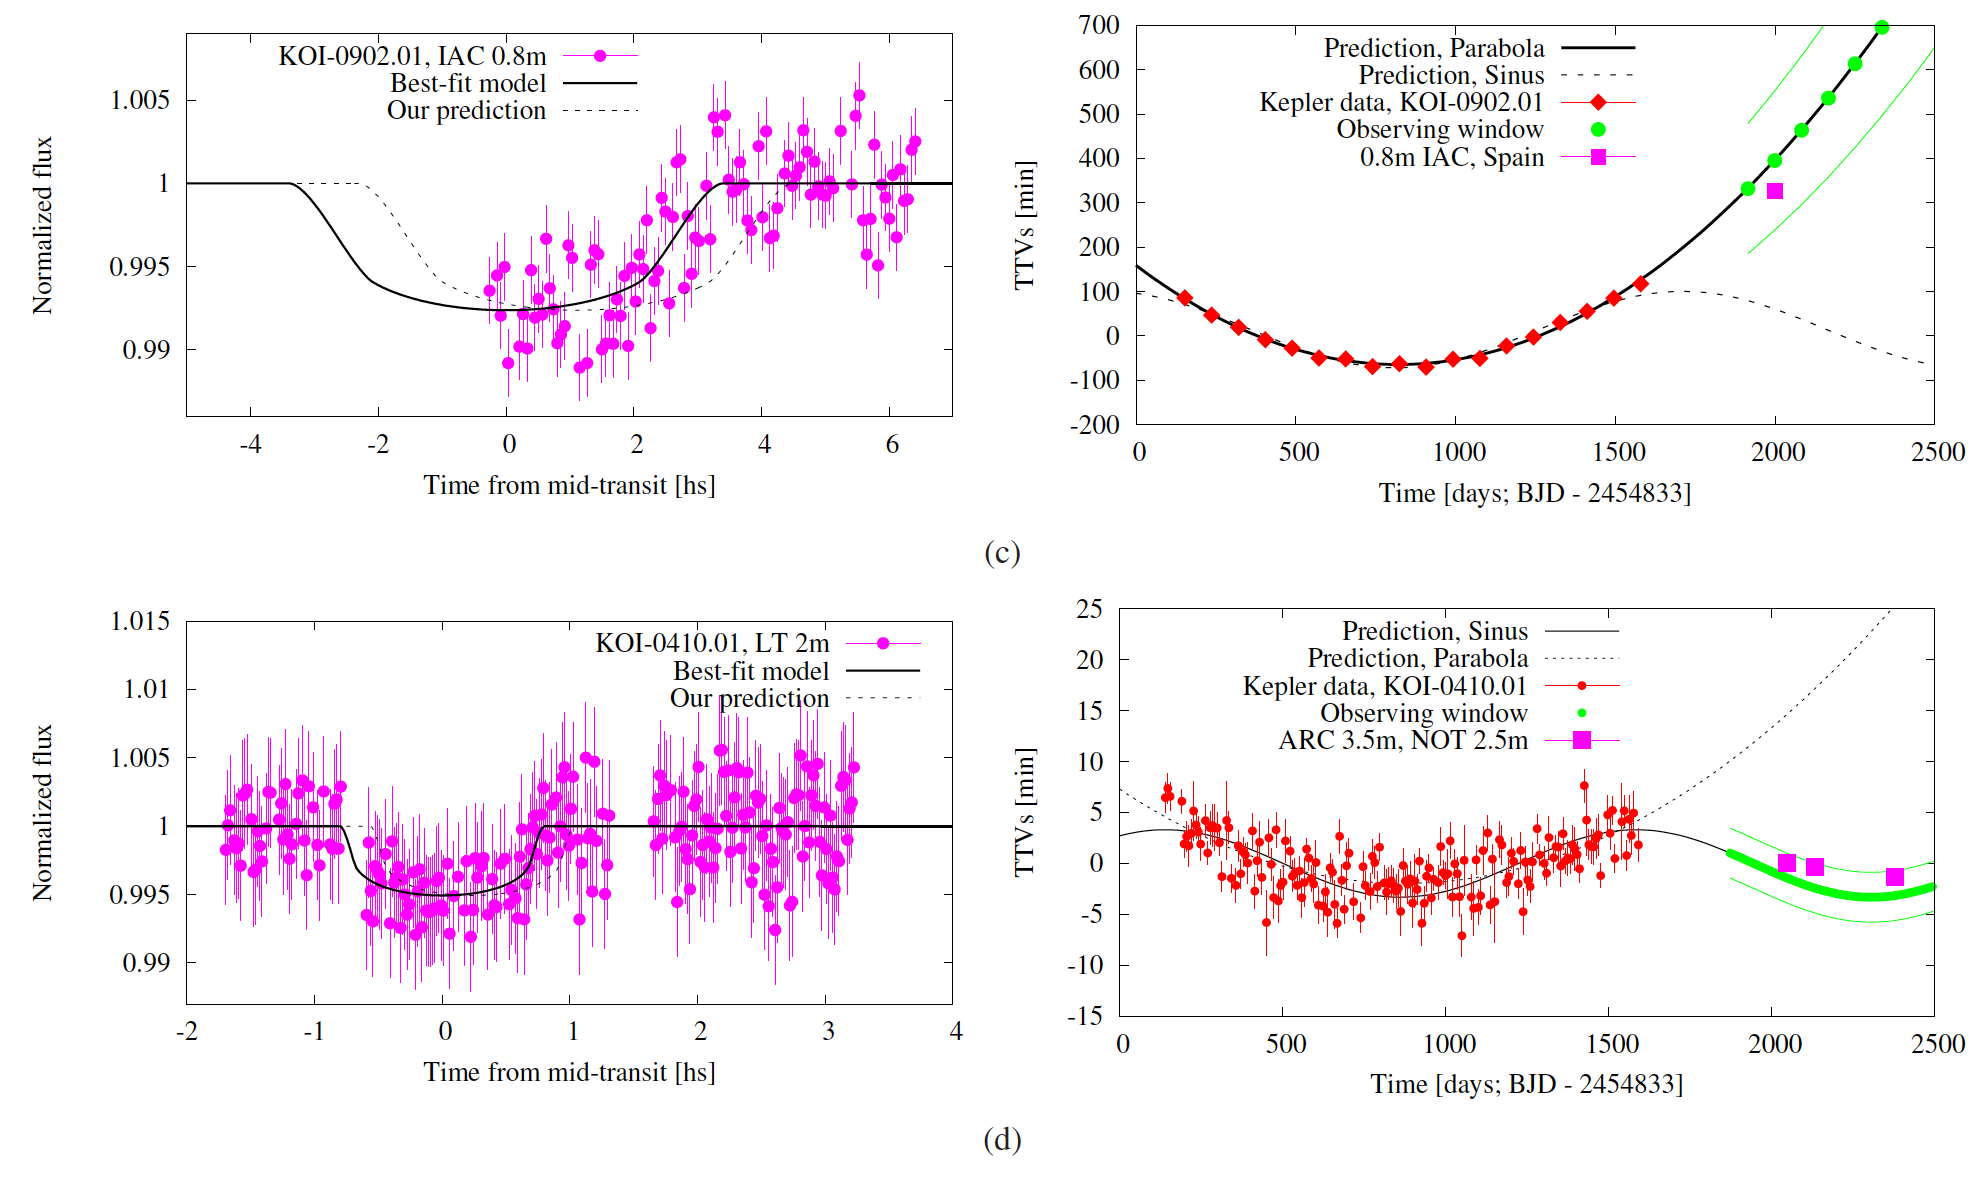
\includegraphics[scale=0.23]{koinet/caro2.png}
    \caption{This figure is reproduced from \citet{vonEssen2018}. {\it Left}: From upper left to bottom right in each pair of figures, transit observations of four KOIs in hours with respect to the best-fit mid-transit time, carried out by different telescopes that are part of KOINet. In all cases, pink circles show detrended data, grey squares correspond to raw data, continuous black lines indicate the best-fit transit models and dashed black lines are plotted to show the predicted transit. {\it Right}: From top to bottom, Kepler (red diamonds) and ground-based (pink circles) observed TTVs for the KOIs displayed on the left. Continuous and dashed black lines indicate, when required, the shape of the two different predictions. In green points the predictions for the first two campaigns are plotted, along with their computed uncertainties.}
    \label{fig:koinet}
\end{figure}

Small habitable planets are usually found via the transit method, since the radial velocities that they impart on their host stars are very small. The transits of these small worlds reveal their radii, and we may be able to deduce their masses and therefore bulk densities using transit timing variations (TTVs) if there are other planets in the system \citep{Agol2005, Holman2005}. As each planet orbits the host star, the gravitational interactions with the other planets in the system impart perturbations on the times of transit as observed from Earth. Precise transit timing measurements can yield constraints on the masses of the planets.

One effort to measure transit timing variations that I have participated in is the KOINet project. This network is led by PI Dr.~Carolina von Essen, who has assembled a team of observers around the world to observe transits of \kepler Objects of Interest (KOIs). She has identified 60 transiting planet candidates that show non-linear transit time ephemerides in \kepler photometry, which indicate that these planet candidates are gravitationally interacting with others in their systems. Further observations of these targets could provide dynamical mass constraints on one or both planets in the system, so the KOINet team is collecting photometry on this subset of the KOIs. These mass constraints allow us to fill out the planetary mass-radius diagram and understand bulk compositions of planets.

Since 2013, I have been the observer for the Apache Point Observatory (APO) node of KOINet. I have observed more than ten transits of KOIs with non-linear transit ephemerides with the Astrophysics Research Consortium (ARC) 3.5 m telescope, using the Agile high-speed photometer \citep{Mukadam2011}. These observations are featured in \citet{vonEssen2018}, and some of the transit times from my APO observations are featured in Figure~\ref{fig:koinet} subplots $b$ and $d$. 

As one of the largest telescopes in the KOINet collaboration, we are tasked with observing the dimmest targets and the targets with the shallowest transits. One such planet is the $5 R_\oplus$ planet orbiting a G star KOI-525, shown in Figure~\ref{fig:koinet}b, with transit depth 0.1\% \citep{Batalha2013}. The \kepler transit photometry for this planet only spanned a fraction of the super-period of the transit timing variations, so an accurate measurement of the super-period was impossible with \kepler photometry alone. The addition of our APO observations enables much better constraints on the TTV super-period, which in turn will provide significantly tighter constraints on the masses of the planets in the system.